\documentclass[UTF8,a4paper,11pt,fontset=fandol]{ctexart}
\usepackage[margin=2cm]{geometry}
\usepackage{amsmath,amssymb,booktabs,graphicx,float,fancyhdr}
\usepackage[hidelinks]{hyperref}
\pagestyle{fancy}\fancyhf{}
\fancyhead[L]{\small INT6165 贝叶斯补充}
\fancyhead[R]{\small 任务 8}\fancyfoot[C]{\thepage}
\setlength{\headheight}{15pt}\setlength{\parskip}{3pt}
\renewcommand{\arraystretch}{1.15}
\begin{document}
\section*{8\quad Beta--二项模型}
\subsection*{模型与先验}
每类访客分别建模，$x$ 为购买会话数，$n$ 为总会话数：
\[
x\mid p\sim\operatorname{Binomial}(n,p),\qquad
p\sim\operatorname{Beta}(a,b).
\]
两组先验独立，似然按独立会话处理。主方案取 $a=b=1$，即 0--1 上的均匀先验，不是从这批数据拟合得到的先验。Jeffreys 先验 $a=b=0.5$ 用于敏感性核对。
\subsection*{共轭更新}
\begin{align*}
\pi(p\mid x,n)&\propto p^x(1-p)^{n-x}p^{a-1}(1-p)^{b-1}\\
&=p^{a+x-1}(1-p)^{b+n-x-1},\\
p\mid x,n&\sim\operatorname{Beta}(a+x,b+n-x),\\
\mathbb E[p\mid x,n]&=\frac{a+x}{a+b+n}.
\end{align*}
95\% 等尾后验可信区间（CrI）取后验分布的 2.5\% 与 97.5\% 分位数，采用 \texttt{scipy.stats.beta.ppf} 计算。
\subsection*{Beta(1,1) 主方案结果}
\begin{center}\small
\begin{tabular}{llrl}
\toprule 访客 & 后验分布 & 后验均值 & 95\% 等尾 CrI\\ \midrule
新访客 & $\mathrm{Beta}(423,1273)$ & 24.94\% & [22.91, 27.03]\% \\
回访者 & $\mathrm{Beta}(1471,9082)$ & 13.94\% & [13.28, 14.61]\% \\
\bottomrule\end{tabular}\end{center}
例如新访客有 422 次购买、1,272 次未购买，后验为
\[
\operatorname{Beta}(1+422,1+1272)
=\operatorname{Beta}(423,1273).
\]
此模型比较总体两组购买率，\textbf{没有按浏览量调整}，不能替代任务 7 的分组结果或回归。
\newpage
\section*{8\quad 后验区间与两组差值}
\begin{figure}[H]\centering
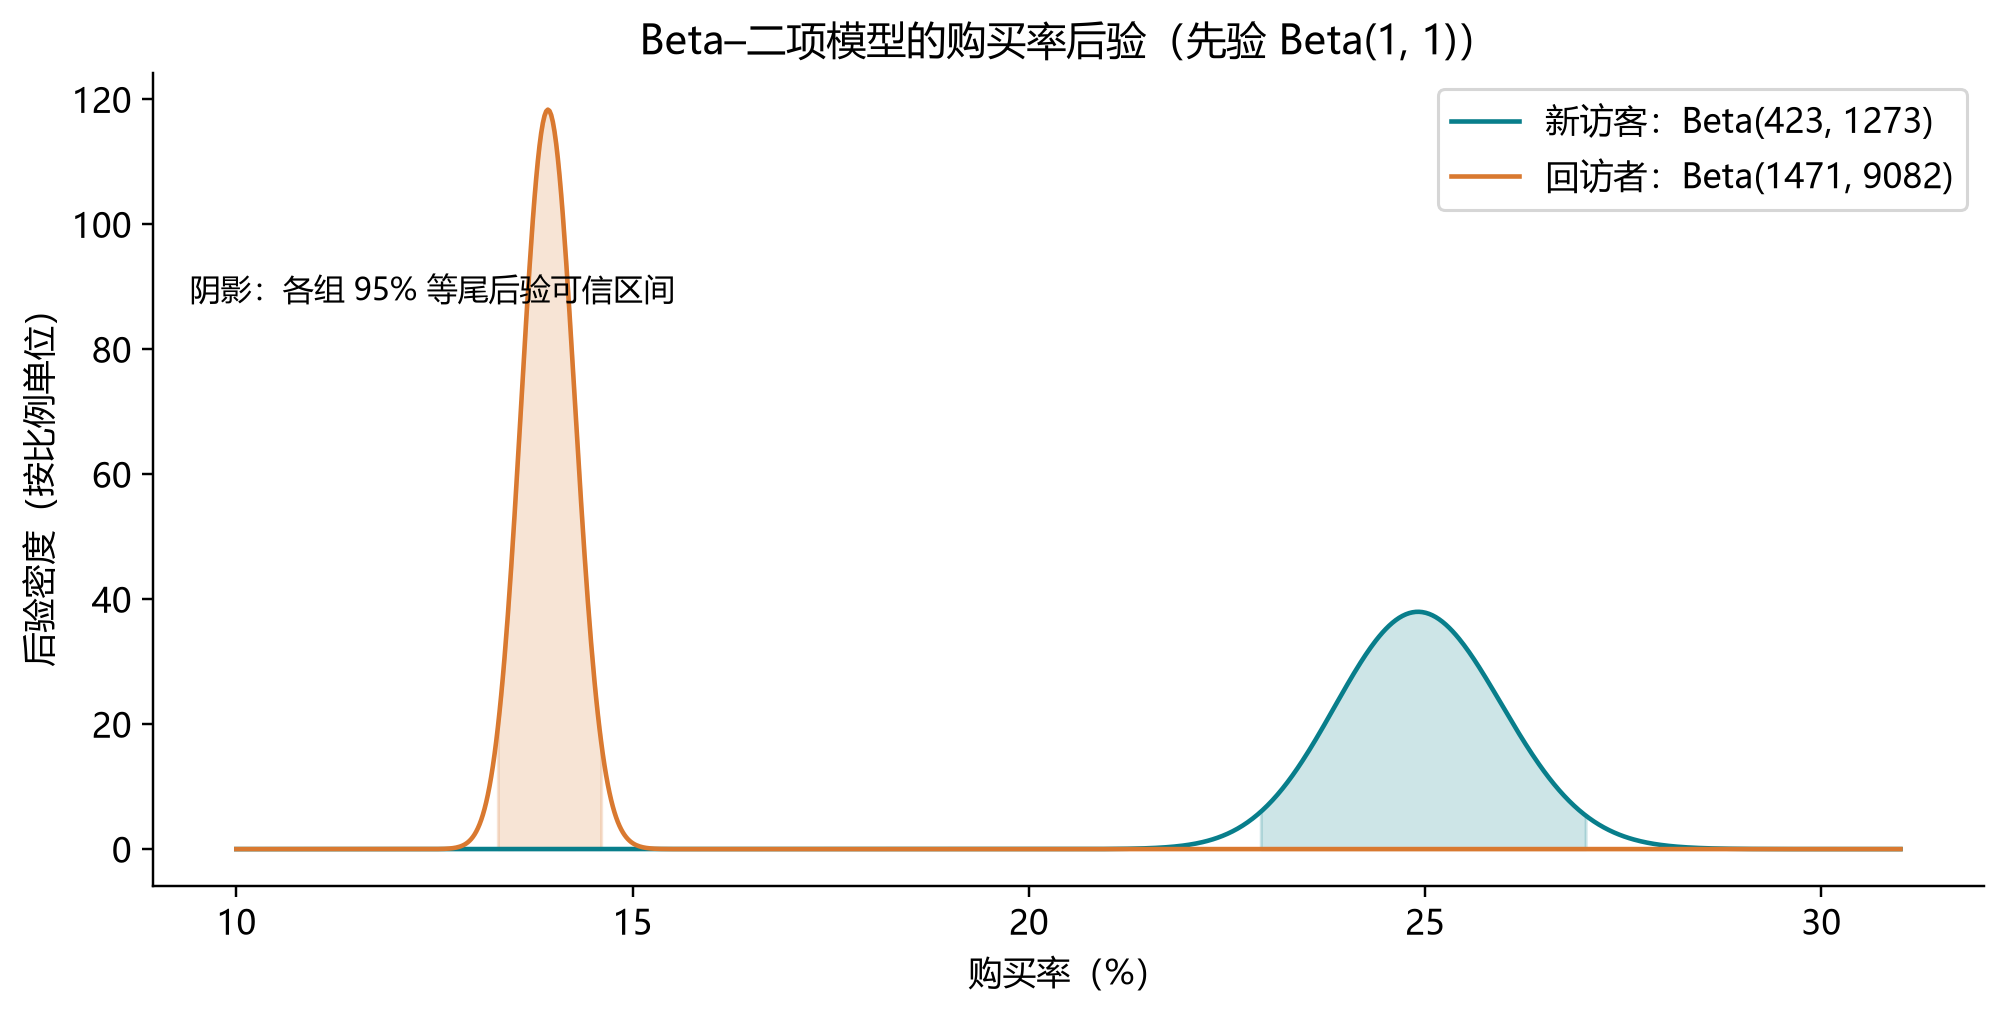
\includegraphics[width=.88\linewidth]{figures/08_posterior_densities.png}
\caption{两组后验密度；阴影为各自 95\% 等尾可信区间}
\end{figure}
设 $\Delta=p_{\mathrm{N}}-p_{\mathrm{R}}$，利用两组后验独立性：
\[
F_{\Delta}(d)=\int_0^1 f_{\mathrm{R}}(r)
F_{\mathrm{N}}(r+d)\,\mathrm{d}r.
\]
通过数值积分与求根获得差值分位数，不相减单组区间。另以固定种子 20261124 的一百万次后验抽样核对区间。

主方案下差值后验均值为 \textbf{11.00 个百分点}，95\% 等尾 CrI 为 \textbf{[8.86,13.19] 个百分点}。
\begin{figure}[H]\centering
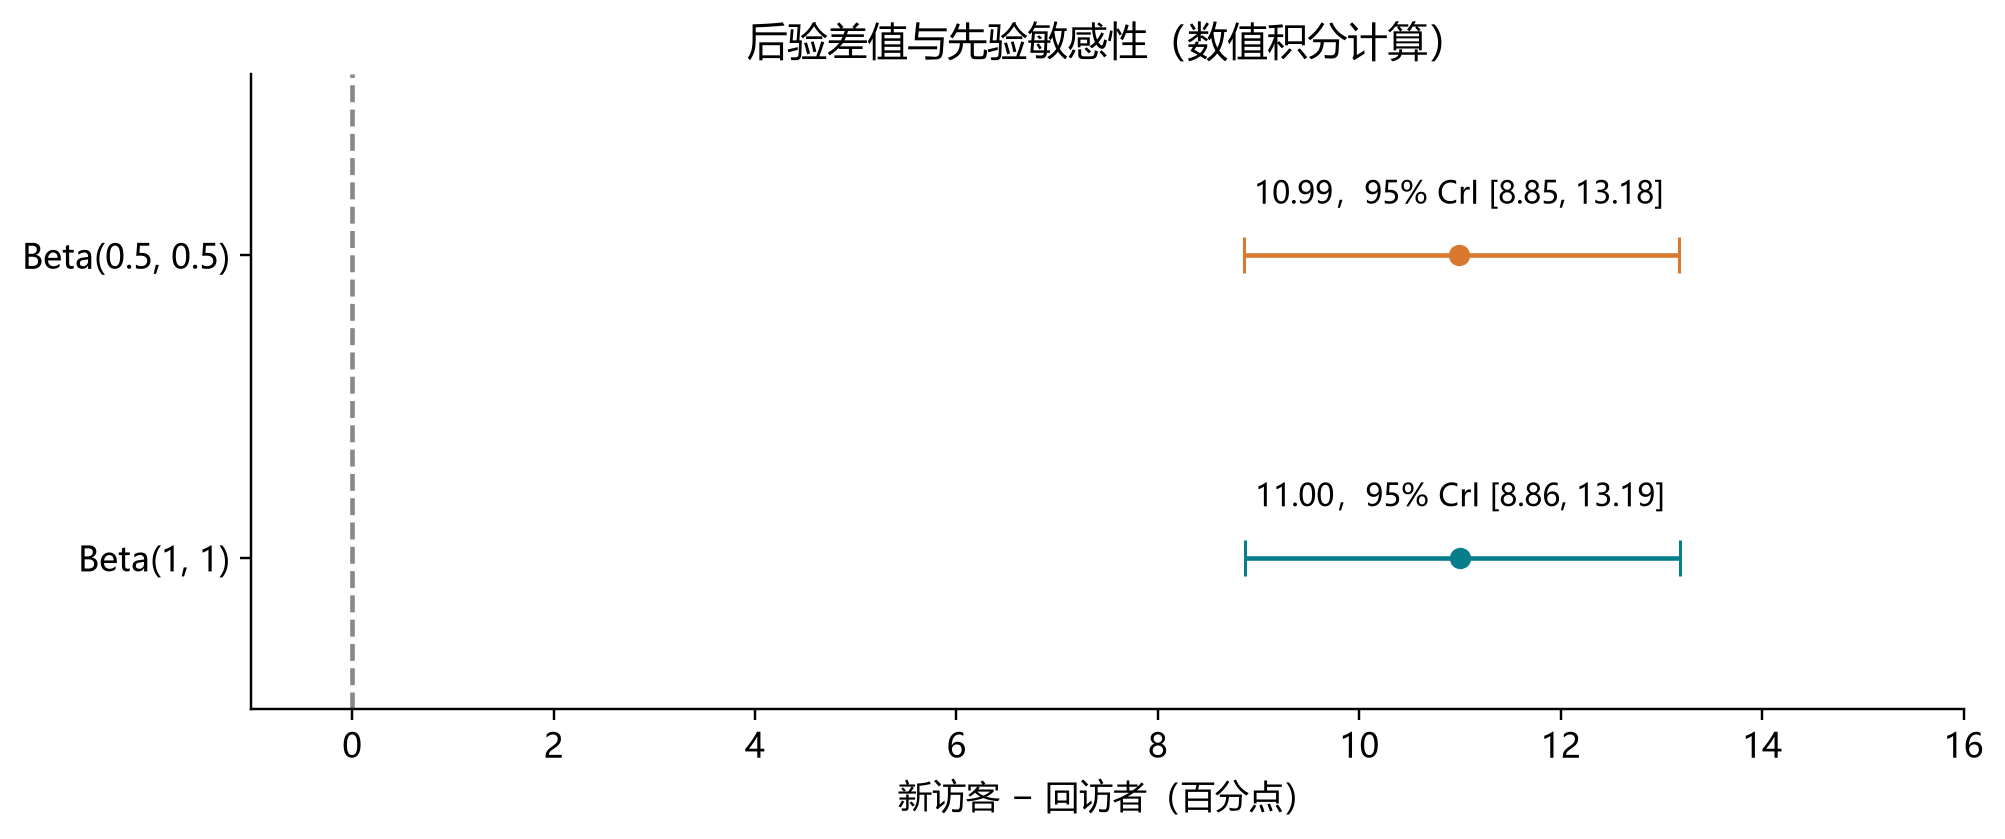
\includegraphics[width=.88\linewidth]{figures/08_posterior_difference.png}
\caption{两种先验下的差值后验均值与 95\% 等尾 CrI}
\end{figure}
主方案下，
$P(p_{\mathrm{N}}\le p_{\mathrm{R}}\mid\text{数据})\approx2.1138\times10^{-28}$，
故 $P(p_{\mathrm{N}}>p_{\mathrm{R}}\mid\text{数据})>99.9999\%$。
这不是频率学派的 $p$ 值，不应因舍入而写成“100\% 确定”。
\newpage
\section*{8\quad 先验敏感性与展示解释}
\begin{center}
\begin{tabular}{lrr}
\toprule 两组共同先验 & 差值均值（百分点） & 95\% 等尾 CrI（百分点）\\ \midrule
Beta(1,1) & 11.00 & [8.86, 13.19] \\
Beta(0.5,0.5) & 10.99 & [8.85, 13.18] \\
\bottomrule\end{tabular}\end{center}
两种弱先验给出的方向、量级接近，未穷尽其他先验。此前频率分析的差值为 10.98 个百分点，95\% 置信区间为 [8.82,13.14] 个百分点。贝叶斯结果与之接近，但使用\textbf{同一批数据}，不能视为独立样本的重复验证。
\subsection*{可信区间与置信区间}
给定先验、模型和数据，参数落在当前 95\% 后验可信区间的后验概率为 95\%。频率学派置信区间描述反复抽样时区间构造程序的长期覆盖率，两者含义不同。
\subsection*{展示前应能回答}
\begin{enumerate}
\item \textbf{为什么用 Beta？}它定义在 0--1 上，可表达对购买率的不确定性，且与二项似然共轭。
\item \textbf{参数怎样更新？}先验参数分别加购买数、未购买数。主方案新访客为 Beta(423,1273)，回访者为 Beta(1471,9082)。
\item \textbf{区间说明什么？}给定先验、模型和数据，对未知购买率或差值的后验不确定范围，不是会话结果的取值范围。
\item \textbf{能否证明因果？}不能。数据是观察性的，独立性无法完全验证，未控制其他因素，贝叶斯方法也不自动消除这些限制。
\end{enumerate}
\subsection*{复核与限制}
后验分位数通过 CDF 检查，差值区间经模拟核对，反向概率以两种等价积分核对。

样本并非已知的随机抽样。125 条重复记录保留。会话相关性或模型设定偏差会影响区间和概率解释。结论限于当前数据及所用假设。
\subsection*{方法参考}
\begin{itemize}
\item \href{https://docs.scipy.org/doc/scipy/reference/generated/scipy.stats.beta.html}{SciPy：Beta 分布及分位数计算}。

\item \href{https://mc-stan.org/docs/stan-users-guide/efficiency-tuning.html\#exploiting-conjugacy}{Stan 用户指南：共轭计算}。
\end{itemize}
\end{document}
